\section{System Overview}
\label{sec:system}

CodeGraph formulates repository retrieval as a staged transformation from raw source code to ranked context. The pipeline comprises parsing, graph construction, seed selection, PPR-based ranking, and context delivery. \Cref{fig:pipeline-architecture} illustrates this workflow. By separating graph construction (offline) from retrieval (online), the system guarantees deterministic, low-latency responses suitable for agent integration.

\begin{figure}[htbp]
    \centering
    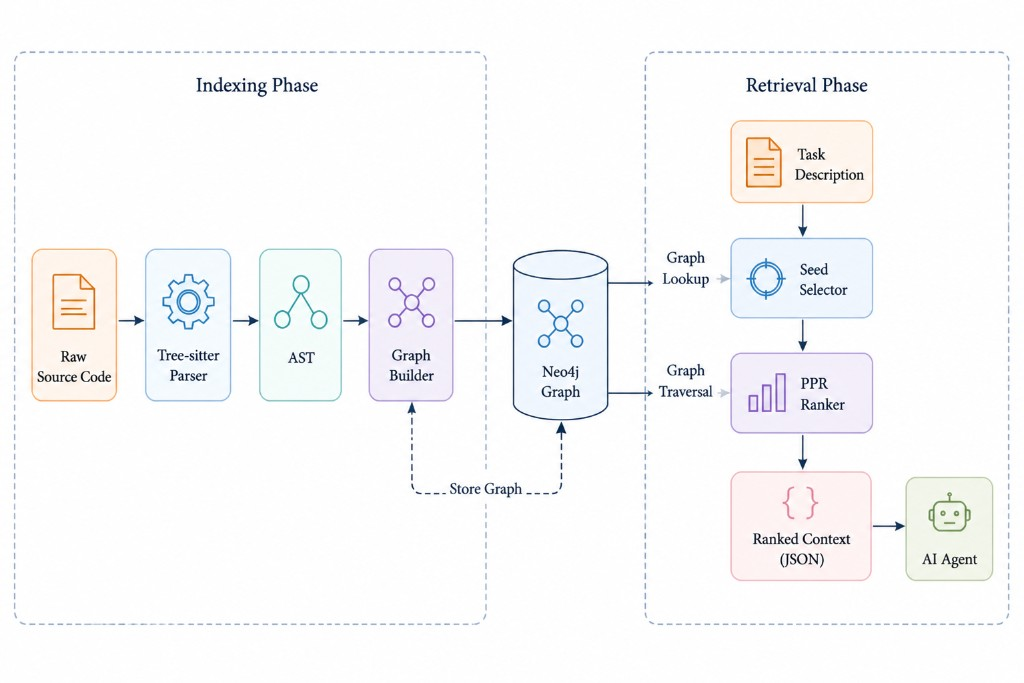
\includegraphics[width=\linewidth]{assets/pipeline_architecture.png}
    \caption{CodeGraph indexing and retrieval pipeline. The indexing phase builds the repository graph offline; the retrieval phase ranks context per query for the AI agent.}
    \label{fig:pipeline-architecture}
\end{figure}

\subsection{Graph Representation}

Graph-based retrieval requires an explicit structural representation of the repository. CodeGraph uses Tree-sitter \cite{treesitter} to extract a four-entity model: files, classes, functions, and methods. This granularity captures the units through which Python code is typically referenced while preserving a graph size that remains efficient for matrix operations.

CodeGraph stores these entities as a property graph in Neo4j \cite{neo4j2024docs}, using four edge types (\texttt{CONTAINS}, \texttt{CALLS}, \texttt{IMPORTS}, and \texttt{INHERITS\_FROM}) to capture the main structural patterns of a Python codebase (\Cref{fig:graph-schema}). Call resolution favors precision over recall by omitting ambiguous call sites, ensuring that graph pathways reflect genuine structural dependencies rather than false positive links.

\begin{figure}[htbp]
    \centering
    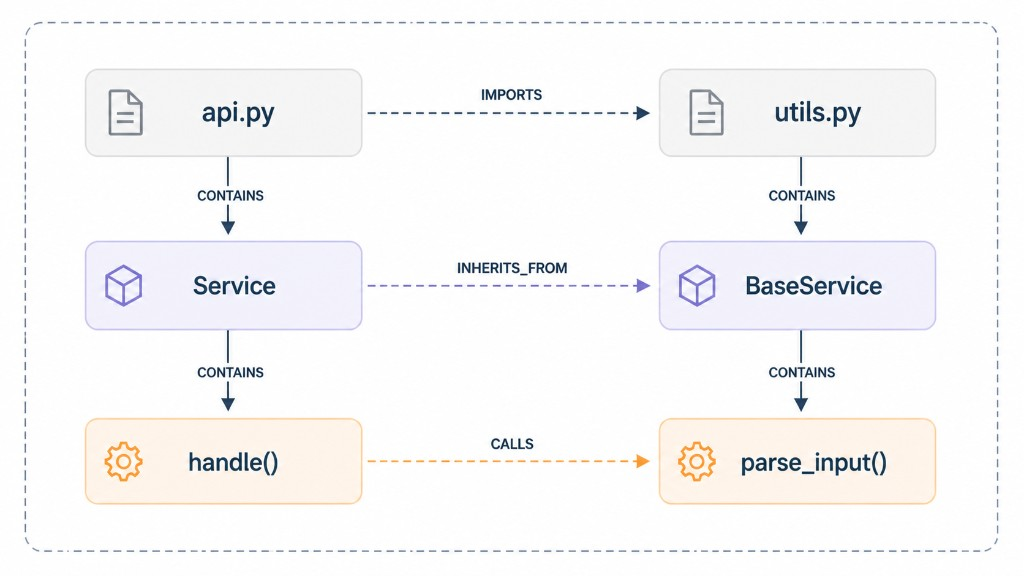
\includegraphics[width=\linewidth]{assets/graph_schema.png}
    \caption{CodeGraph property-graph schema. Nodes represent fundamental code units; edges capture containment, linkage, extension, and invocation.}
    \label{fig:graph-schema}
\end{figure}

\subsection{Context Delivery}

Once the PPR algorithm ranks the graph, the result must be packaged into a fixed context budget. CodeGraph post-processes the ranked nodes by deduplicating entities from the same file, dropping parent \texttt{File} nodes if specific sub-entities (like a method) are already highly ranked, and extracting the corresponding source text. 

The entire retrieval pipeline is wrapped into a Model Context Protocol (MCP) server. This exposes a single \texttt{get\_relevant\_context} tool, allowing AI agents to programmatically fetch ranked, budget-constrained source snippets deterministically, avoiding the latency and instability of LLM-generated graph queries inside the retrieval loop.
